\documentclass{article}


\usepackage{fullpage}
\usepackage{amsfonts}
\usepackage{amssymb,amsmath,amsthm}
\usepackage{algorithm,algorithmic}
\usepackage{graphicx}

\newtheorem{thm}{Theorem}

\def\R{\mathbb{R}}
\def\E{\mathbb{E}}
\def\Mult{\mathbf{Mult}}
\def\Cat{\mathbf{Cat}}
\def\Dir{\mathbf{Dir}}
\def\spn{\mathbf{span}}
\def\diag{\mathbf{diag}}
\def\ones{\mathbf{1}}


\title{CSE291 Report: Topic Discovery using Nonnegative Matrix Factorization under Separability assumption}
\author{Chicheng Zhang}

\begin{document}
\maketitle

\section{Problem Setting}
\subsection{Topic Discovery: Generative Model}
Throughout the report, we assume the following generative model of corpus: Suppose the topic matrix $A$ is fixed, each column of $A$ is a topic(sports, technology, etc), i.e. a discrete distribution over a $n$-word vocabulary. for each document $D_i, i = 1, \ldots, m$, the topic proportion $\theta_i \sim T$, $T$ is a distribution over $\Delta^{k-1}$, e.g. $\Dir(\alpha)$. Then the $j^{th}$ word $w_{ij}$ are generated by a categorical ditribution $\Cat(A\theta_i)$, $j = 1 ,\ldots, N_i$, where $N_i$ is the number of words in document $i$, i.e. $w_{ij} = e_k$ if $w_{ij}$ is the $k^{th}$ word in vocabulary. Our goal is:

\framebox[0.9\textwidth]{Given a corpus $C = \{ D_i, i = 1, \ldots, m \}$, recover the topic matrix $A$. }


\subsection{Tool: (Approximate)Nonnegative Matrix Factorization}
\label{tool:nmf}
Suppose a matrix $M \in \R^{a \times b}$, $M \ge 0$ entrywise, assume it can be factorized as $M = FW$, $F \in \R^{a \times r}$, $W \in R^{r \times b}$, $F,W \ge 0$ entrywise. Given a corrupted version of $M$, i.e. $\hat{M}$, each row $|\hat{M}^i - M^i| \le \epsilon$, our goal is to find $\hat{F},\hat{W} \ge 0$ such that $\forall i,j, (\hat{F} - F)_{ij}, (\hat{W} - W)_{ij} \le f(\epsilon)$ for some function $f$. As we shall see next, the technique of solving nonnegative matrix factorization can be used in topic discovery problem.

\subsection{Separability Assumption}
Given $M = FW$, separability assumption says for each column $i$ of $F$, there is a row $F^{f(i)}$ such that it is nonzero only in column $i$. Moreover we call it $p$-separable if the entry $F_{f(i),i}$ is greater than $p$. From NMF's perspective, if separability is not assumed, the factorization solution can be not unique. Further discussion of the assumption is provided in subsection~\ref{disc:sep}.

\subsection{Which Matrix to Factorize?}
Given the corpus $C$, there are two natural choice of factorization:

The first choice is $\hat{M}_1 \in \R^{n \times m}$, whose row $i$ containing the average word frequency of document $i$, i.e. $\sum_j w_{ij}/ N_i$. It can be seen that $\E(M_1|\theta_1, \ldots, \theta_m) = A(\theta_1, \ldots, \theta_m)$. we can recover $A$ based on $\hat{M}_1$. Unfortunately this direct approach suffers from noise too much, since if $N_i$ are small, each entry of $\hat{M}_1$ is also noisy. As $m \to \infty$, it cannot guarantee consistency of estimation of $A$. 

The second choice is the Gram matrix $\hat{M}_2 = \hat{\E}(w_1 w_2^T) \in \R^{n \times n}$, which characterizes word-word correlation within a document. As the number of document increases, the empirical estimate $\hat{\E}(w_1 w_2^T) \rightarrow \E(w_1 w_2^T)$. Note in this approach as long as $N_i \ge 2$, if $m \to \infty$, we are still able to recover $A$. Under the generative model defined above, $\E(w_1 w_2^T) = ARA^T$, where $R = \E(\theta_i \theta_i^T)$, Taking $M = ARA^T$, $F = A \in \R^{n \times k}$, $W = RA^T \in \R^{k \times n}$ in subsection~\ref{tool:nmf}, the topic discovery problem reduces to recover $A$ with access to a noisy version of $M$, assuming $A$ is separable. It is argued that the separabilty assumption holds in real corpus: for example, "kobe\_bryant" is likely to appear only in topic of basketball, "bunt" is likely to appear only in topic of baseball, etc, and these are often called "anchor" words.

\section{Literature Overview}
\subsection{NMF under Separability Assumption}
Recently \cite{AGKM12} open a new avenue of NMF, relying on separability assumption. The intuition is described as follows. Observe that under separability assumption, after normalizing each row of $M$, the convex hull of rows is simple -- a $r$-dimensional simplex. Then we can recover $F$ and $W$ approximately using a two-stage algorithm: first find the vertices of the convex hull of rows based on linear programming(finding robust loners), then they are the perturbed version of a permutation of rows of $W$. Then solve the constrained optimization problem $\min_{\hat{F}} ||\hat{M}-\hat{F}\hat{W}||_1$ to obtain $\hat{F}$. \cite{BRRT12} solve the problem based on localizing factorization, using a single linear program involving $n \times n$ variables, which they argue can be solve fastly by incremental gradient descent. \cite{KSK12} proposed some heuristic to find the vertices, based on unnormalized $M$, and found extreme rays of $M$ based on repeat detection and projection. 

\subsection{Application to Topic discovery}
\cite{AGM12,AGH+13} tailored the NMF algorithm to topic discovery problem. \cite{AGM12} improved upon the previous work using more delicate definition of robust loner, and used matrix inversion to recover $A$ and $R$. \cite{AGH+13} presents a combinatorial algorithm to find vertices, hence finding $W$, then use Bayes' Theorem to recover $A$, which is more robust than the inversion approach. Our implementation is mainly based on this line of work. \cite{DRIS13} proposed to find anchor rows using data dependent projection/random projection, but relies on an unnatural quantity $\beta_{\wedge}$ (the lower bounds of non-zero elements of $A$).

\section{Implementation}
In our implemetation we only conducted experiments on \cite{AGH+13}, since it has both solid theoretical guarantees and practical. To construct the empirical cross word moment matrix we use:
$$
\hat{M} = \hat{\E}(w_1 w_2^T) = \frac{1}{m}\sum_{i=1}^{m}\frac{1}{|N_i|(|N_i|-1)}(c_i c_i^T - \diag(c_i))
$$
where $c_i = \sum_{j=1}^{N_i} w_{i,j}$ is the count of words in document $i$.
It can be seen that
$$
\hat{M} \overset{p}{\to} \E(w_1 w_2^T) = \E(\E(w_1  w_2^T|\theta))= A\E(\theta \theta^T)A^T = A \cdot RA^T = A \cdot W
$$

\subsection{Finding Anchor Rows}
Suppose we get the true $M = AW$, we normalize each row of $M$,$A$,$W$; denote $\bar{M} = \diag(M \ones)^{-1} M$, $\bar{A} = \diag(M \ones)^{-1} A \diag(W \ones)$, $\bar{W} = \diag(W \ones)^{-1} W$ as the row-normalized version respectively. A simple observation yields that $\bar{M} = \bar{A}\bar{W}$. The row $f(i)$ corresponding anchor words for topic $i$, of $\bar{A}$ is (0,\ldots,0,1,0,\ldots,0), so the row $f(i)$ of $\bar{M}$ stores exactly a copy of $\bar{W}^i$. Moreover, non-anchor rows are within the convex hull of $\bar{W}^i$, since $\forall j$, $\bar{M}^j = \sum_{i=1}^k \bar{a}_{ij} \bar{W}^j$. In other words, the rows of $\bar{M}$ lies within a simplex with vertices $\bar{M}^{f(i)}, i = 1, \ldots, k$. Moreover if the $A$ is $p$-separable and $R$'s $\ell_1$-condition number is lower bounded by $\gamma$, then $W = RA^T$ is $O(\gamma p)$ robustly simplicial, i.e. the $\ell_2$ distance of any $\bar{W}^i$ to the convex hull of $\{ \bar{W}^j: j \neq i \}$ is at least $\gamma$. This leads to the robust anchor row finding algorithm~\cite{AGH+13}:

\begin{algorithm}[H]
\caption{Robust Anchor Row Finding}
\begin{algorithmic}[1]
\STATE {\bf{Inputs:}} Gram matrix $\bar{M}$.
\STATE {\bf{Outputs:}} Approximate anchor rows $\{ v'_1, \ldots, v'_k \}$.
\STATE $S = \{M^i\}$ such that $\bar{M}^i$ is the farthest point from the origin
\FOR {$i$ = $1$ to $k-1$}
\STATE    Let $M^i$ be the point in \{$\bar{M}^1$, \ldots, $\bar{M}^n$\} that has the largest distance to $\spn(S)$
\STATE     $S = S \cup \{ \bar{M}^i \}$
\ENDFOR
\STATE $S = \{v_1', \ldots, v_k'\}$
\FOR {$i$ = $1$ to $k$}
\STATE     Let $\bar{M}^j$ be the point that has the largest distance to $\spn(\{v_1', \ldots, v_k'\} \backslash \{ v_i' \})$
\STATE    update $v'_i$ to $\bar{M}^j$
\ENDFOR
\STATE Return $\{ v'_1, \ldots, v'_k \}$
\end{algorithmic}
\end{algorithm}


\subsection{Recover Topic Matrix Using Bayes' Theorem}
The row normalization has a probablistic interpretation: suppose originally $M_{ij} = \Pr(w_1 = i, w_2 = j)$, then 
$$
    \bar{M}_{ij} = \Pr(w_2 = j | w_1 = i) = \sum_k \Pr(w_2 = j | z_1 = k) \Pr(z_1 = k | w_1 = i)
$$
If row $f(k)$ is an anchor row for topic $k$, which means $\Pr(w_1 = f(k) | z_1 = k) > 0$, while $\Pr(w_1 = f(k) | z_1 = l) = 0, l \neq k$, then it implies $\Pr(z_1 = k | w_1 = f(k)) = 1$.
So picking the rows $f(k)$, $\bar{M}_{f(k)j} = \Pr(w_2 = j | w_1 = f(k)) = \Pr(w_2 = j | z_1 = k)$.
Hence we can get $\Pr(z_1 = k | w_1 = i)$ for all $i$, since we have an overdetermined equation:
$$
    \bar{M}_i = \sum_k \Pr(z_1 = k | w_1 = i) \bar{M}_{f(k)}
$$
which has $n$ variables and $k$ equations.
In implementation we solve the least squares problem, as well as ensuring positiveness and normalization of $\Pr(z_1 = k | w_1 = i)$(denote it as $C_{ik}$), i.e.

\begin{align*}
\min & ||\bar{M}_i - C_i^T(\bar{M}_{f(1)}, \ldots, \bar{M}_{f(k)})^T||^2 \\
\text{subject to}  & C_i \ge 0 \\
           & \sum_{i=1}^k C_i = 1 
\end{align*}

Finally using Bayes' theorem, the topic matrix $A$ can be recovered:
$$
A_{ik} = \Pr(w_1 = i | z_1 = k) = \frac{\Pr(z_1 = k | w_1 = i) \Pr(w_1 = i)}{\sum_k \Pr(z_1 = k | w_1 = i) \Pr(w_1 = i)}
$$
where $\Pr(w_1 = i) = \sum_j \Pr(w_1 = i, w_2 = j)$ can be directly obtained in $M$.


\section{Experiments}

\subsection{Real Coupus}
We conducted experiments on New York Times as well as NIPS abstracts corpus. The illustrative results(top words from extracted topics) is provided in appendix~\ref{exp:corpus}.


\subsection{Semi-Synthetic Datasets: Sample Complexity}
We validate the algorithm's sample complexity bound on synthetic corpus. We use a topic matrix $A$ extracted from New York Times corpus $\in \R^{n \times k}$ and use i.i.d. $\theta_i \sim \Dir(0.1,\ldots,0.1)$ to generate topic distribution for each synthetic document. Then for each document $i$ we sample $N_i$ words i.i.d. from $\Cat(A\theta_i)$. Here we use $k = 10, n = 1000$. We set $N_i \equiv 100$, and vary $m$, then validate the $\ell_1$ error of each topic; for simplicity, for each ground truth topic $A_i$, we find the nearest $\ell_1$ neighbor $\hat{A}_j$ and test the value of $||A_i - \hat{A}_j||_1$.

\begin{thm}[Sample Complexity\cite{AGH+13}]
Suppose $m,n,k,\gamma,p$ is defined as above, $N_i \equiv N$, $a = \max_{i,j} \E(\theta_j)/\E(\theta_i)$ is the topic imbalance, then $\forall \epsilon > 0$
$$
    m \geq O(\frac{ak^3\log n}{N(\gamma p)^6 \epsilon}), O(\frac{(ak)^3 \log n}{N (\gamma p)^4 \epsilon^3})
$$
the algorithm learns $A$ matrix with entry wise error at most $\epsilon$.
\end{thm}

Since in our ground truth $A$ is not perfectly separable, we do not expect the error dropping to $0$ as $m \to \infty$. The $\ell_1$ error of all 10 topics extracted wrt varying $m$ are depicted as follows: 
\begin{figure}[h]
\centering
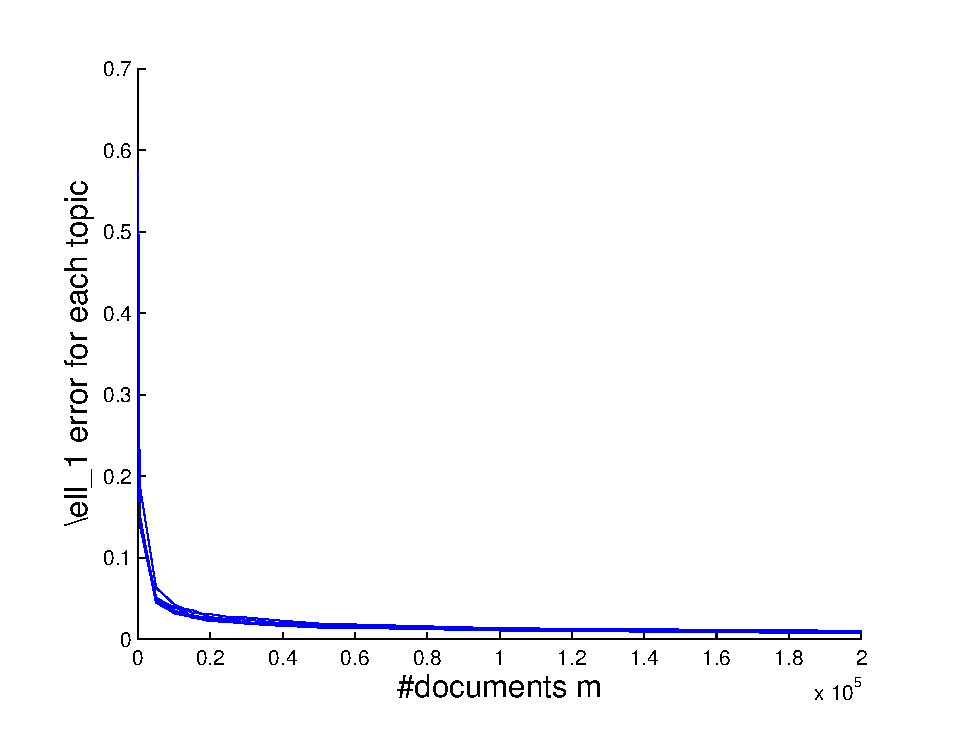
\includegraphics[width=0.5\linewidth]{../code/sc.eps}
\end{figure}

\section{Discussion}

\subsection{Is Separability Assumption Reasonable?}\label{disc:sep}
\cite{DS03} argues that separability assumption holds commonly in image segmentation, and \cite{AGKM12} also claims it is met in topic modelling, moreover there can be several anchor words for one specific topic. But in some cases it is not quite natural: suppose we expect to extract a "overview" topic, whose support spreads widely over words, since there may be non-negligible fraction of survey articles in the corpus. Then under this assumption this is impossible since it does not have its anchor word. \footnote{Thank Akshay Balsubramani for pointing this out.}

Another reason of proposing separablity may be from multiple solutions of the original problem. Suppose $M \in \R^{n \times m}$ can be factorized as products of three nonnegative matrices: $M = A R W$, $A \in \R^{n \times r}, R \in \R^{r \times r}, W \in \R^{r \times m}$, then obviously the rank $r$ nonnegative factorization is not unique: either $AR \cdot W$ or $A \cdot RW$.

\subsection{Comparison with SVD Approach}
Note a big difference between \cite{AGKM12} and \cite{AGH+13} and traditional approach \cite{BNJ03} is that it treats topic discovery a recovery problem: assuming the data are generated from a model, then recover the parameters of the model approximately, while traditional approach focus on building a model, then find the parameters that best fits the training examples, such as MAP estimate. Another recent work \cite{AHK+12} share the principle with the former, using combination of second order moments and third order moments. For constructing their moments, it must assume the topic combination of each documents satisfies some distributional assumptions, such as Dirichlet, which is a stronger assumption, hence it is not surprising that their model may not have so good performance when topics have strong correlation. On the other hand, it does not require the existence of anchor words of each topic.

\bibliographystyle{plain}
\bibliography{nmf}


\appendix
\section{Illustrative Results}
\label{exp:corpus}
Here we present experimental results on anchor words and the top 10 entry in each topic, i.e. each column of $A$ recovered. New York Times Corpus: 

\subsection{New York Times}
\hspace{-2cm}
  \begin{tabular}{ l | l }
    \hline
    \bf{anchor words} & \bf{top 10 words}\\ \hline
    zzz\_tiger\_wood & zzz\_tiger\_wood shot player tour play round win tournament hole course \\ \hline 
    zzz\_kobe\_bryant & point zzz\_kobe\_bryant zzz\_laker shot half quarter lead left scored team \\ \hline 
    cat & cat park animal county owner group restaurant problem food police \\ \hline 
    teaspoon & cup teaspoon minutes tablespoon pepper add sugar pan chicken serving \\ \hline 
    stem & cell stem human research blood scientist egg system skin patient \\ \hline 
    zzz\_microsoft & zzz\_microsoft company window software computer system court operating case product \\ \hline 
    zzz\_israeli & zzz\_israeli palestinian zzz\_israel attack israelis killed zzz\_west\_bank soldier army military \\ \hline 
    zzz\_john\_mccain & zzz\_john\_mccain campaign zzz\_george\_bush republican zzz\_bush political zzz\_party primary zzz\_republican voter \\ \hline 
    zzz\_enron & zzz\_enron company lay energy stock board companies partnership fund trading \\ \hline 
    zzz\_met & zzz\_met team player fan season million baseball night agent free \\ \hline 
    touchdown & yard game play touchdown season point defense quarter quarterback ball \\ \hline 
    zzz\_governor\_bush & zzz\_governor\_bush zzz\_new\_york point plan meeting lead anti record attack zzz\_texas \\ \hline 
    recount & ballot election zzz\_florida recount votes vote court board law voter \\ \hline 
    zzz\_fed & percent economy rates zzz\_fed market rate prices interest economic cut \\ \hline 
    zzz\_dodger & zzz\_dodger season right manager games play start left game home \\ \hline 
    priest & priest abuse church sexual allegation victim official zzz\_boston children child \\ \hline 
    butter & butter food add cup flavor chopped chef minutes green makes \\ \hline 
    anthrax & anthrax mail letter building official office worker found test investigator \\ \hline 
    king & king goal game team play games shot period point minutes \\ \hline 
    gay & gay right parent women group family children member mother child \\ \hline 
    wine & wine red white french list restaurant taste expert www room \\ \hline 
    zzz\_taliban & zzz\_taliban zzz\_afghanistan official zzz\_u\_s military forces government afghan war bin \\ \hline 
    beer & beer chicken skin hour body hand right wood half inside \\ \hline 
    zzz\_at & company companies zzz\_at percent cable customer billion business market plan \\ \hline 
    zzz\_usc & team zzz\_usc game player coach season guy play defense games \\ \hline 
    zzz\_vicente\_fox & zzz\_mexico president zzz\_united\_states government zzz\_u\_s official program zzz\_clinton drug zzz\_vicente\_fox \\ \hline 
    zzz\_medicare & zzz\_bush drug program plan zzz\_medicare bill benefit zzz\_congress billion cost \\ \hline 
    teacher & school teacher student program percent children high parent kid education \\ \hline 
    zzz\_vladimir\_putin & zzz\_russia official zzz\_russian zzz\_vladimir\_putin president government russian military system zzz\_moscow \\ \hline 
    yankees & yankees season team million player zzz\_new\_york games baseball manager pitcher \\ \hline 
    chocolate & chocolate food room find look help com book feel hand \\ \hline 
    zzz\_arthur\_andersen & company case lawyer zzz\_arthur\_andersen money firm government investor statement told \\ \hline 
    zzz\_rudolph\_giuliani & zzz\_rudolph\_giuliani zzz\_new\_york official mayor children president public police decision court \\ \hline 
    zzz\_ford & computer zzz\_ford car program company problem official hour high speed \\ \hline 
    salt & salt children side left wife food husband miles eat pound \\ \hline 
    cuban & zzz\_cuba father zzz\_miami boy official cuban family government zzz\_united\_states son \\ \hline 
    zzz\_eastern & com information question www american daily newspaper web zzz\_eastern sport \\ \hline 
    virus & virus program system computer human window disease mail zzz\_new\_york problem \\ \hline 
    zzz\_china & zzz\_china chinese zzz\_united\_states zzz\_american zzz\_u\_s military government zzz\_beijing official zzz\_japan \\ \hline 
    penalty & death penalty case court law lawyer zzz\_texas execution cases right \\ \hline 
    ranger & ranger season game goal right play games left night point \\ \hline 
    prayer & school prayer student zzz\_god high religious public com faith site \\ \hline 
    album & music song album band show record play hit rock musical \\ \hline 
    zzz\_o\_neal & game zzz\_laker zzz\_o\_neal play games season point player team night \\ \hline 
    zzz\_bruin & zzz\_bruin play zzz\_ucla point game season half left right shot \\ \hline 
    nuclear & nuclear weapon terrorist power attack plant zzz\_bush group bomb scientist \\ \hline 
    zzz\_red\_sox & zzz\_red\_sox team season manager zzz\_boston big baseball hit guy fan \\ \hline 
    jet & jet pick round team draft trade zzz\_miami official zzz\_new\_york plane \\ \hline 
    zzz\_abc & show zzz\_abc network program zzz\_nbc television zzz\_cb night series executive \\ \hline 
    zzz\_oscar & film movie zzz\_oscar actor show award movies won fight director \\ \hline 
    
    
  \end{tabular}

\hspace{-2.5cm}
  \begin{tabular}{ l | l }
    \hline
    \bf{anchor words} & \bf{top 10 words}\\ \hline
    zzz\_government & zzz\_government official right law police security officer court case evidence \\ \hline 
    zzz\_gore & zzz\_bush zzz\_gore president campaign zzz\_white\_house million zzz\_republican republican democratic percent \\ \hline 
   firefighter & firefighter building fire zzz\_new\_york family official police officer home found \\ \hline 
    zzz\_aol & web com zzz\_aol mail online zzz\_internet site program internet www \\ \hline 
    index & percent stock market companies fund point index investor average high \\ \hline 
    zzz\_navy & zzz\_navy military room computer system information ship civilian water program \\ \hline 
    zzz\_india & zzz\_india zzz\_pakistan group attack official government zzz\_united\_states terrorist million military \\ \hline 
    zzz\_mccain & campaign zzz\_bush zzz\_mccain zzz\_republican republican zzz\_senate bill vote political voter \\ \hline 
    zzz\_palestinian & official zzz\_palestinian security plan officer forces police zzz\_cia proposal settlement \\ \hline 
    medal & zzz\_olympic medal women run won win gold games zzz\_u\_s final \\ \hline 
    fish & fish water river word small put scientist home boat www \\ \hline 
    zzz\_iraq & zzz\_iraq zzz\_bush zzz\_u\_s war zzz\_united\_states zzz\_american oil military weapon attack \\ \hline 
    zzz\_black & percent zzz\_black black white film group american student part look \\ \hline 
    privacy & information government companies privacy law company mail web computer zzz\_internet \\ \hline 
    zzz\_ncaa & team season game player point games coach tournament play zzz\_ncaa \\ \hline 
    racing & race car driver team won racing track season win start \\ \hline 
    bird & bird light building zzz\_new\_york million book water look night winter \\ \hline 
    starring & film movie minutes hour play starring director character movies actor \\ \hline 
    cancer & women patient cancer drug test doctor percent treatment study disease \\ \hline 
    airline & flight passenger airline percent airport security ticket government business airlines \\ \hline 
    tax & tax percent cut million taxes income money plan pay spending \\ \hline 
    zzz\_al\_gore & zzz\_al\_gore campaign zzz\_george\_bush president democratic presidential voter zzz\_clinton zzz\_texas vice \\ \hline 
    zzz\_giant & team player season zzz\_giant coach play league games zzz\_nfl guy \\ \hline 
    union & union worker government member labor percent official job leader president \\ \hline 
    rocket & team rocket game point season high play shot plan million \\ \hline 
    auction & site million auction company web house zzz\_internet com money stock \\ \hline 
    italian & italian restaurant zzz\_new\_york food show american zzz\_italy part century owner \\ \hline 
    soccer & player team play game soccer goal zzz\_u\_s games women fan \\ \hline 
    con & company companies deal customer power agreement player president statement business \\ \hline 
    cent & company million percent quarter cent analyst share billion sales price \\ \hline 
    zzz\_dick\_cheney & president zzz\_dick\_cheney zzz\_george\_bush administration zzz\_bush zzz\_white\_house military republican zzz\_clinton defense \\ \hline 
    gun & gun law officer police children court right case control violence \\ \hline 
    flag & flag white red black blue vote member right bill american \\ \hline 
    zzz\_yasser\_arafat & palestinian zzz\_yasser\_arafat zzz\_israel peace leader israeli zzz\_bush violence government arab \\ \hline 
    protein & protein human memory brain problem companies scientist food research drug \\ \hline 
    jew & jew jewish zzz\_israel religious group zzz\_american american show war history \\ \hline 
    zzz\_fbi & official zzz\_fbi attack terrorist law investigation case agent information federal \\ \hline 
    birthday & birthday song school family company home mother mail holiday wife \\ \hline 
    chip & chip computer art web com design need mail software technology \\ \hline 
    dog & dog show history house told student book friend family home \\ \hline 
    zzz\_iran & government zzz\_iran political country war zzz\_afghanistan right nation women american \\ \hline 
    patriot & million patriot season player game coach team play quarterback zzz\_nfl \\ \hline 
    publisher & book author publisher writer word right magazine sales published newspaper \\ \hline 
    zzz\_bill\_clinton & zzz\_bill\_clinton president zzz\_george\_bush zzz\_white\_house political office term presidential zzz\_american republican \\ \hline 
    zzz\_aid & drug million zzz\_aid percent government official study patient zzz\_united\_states money \\ \hline 
    farmer & farmer bill farm program government percent food country water billion \\ \hline 
    bankruptcy & million company companies bankruptcy executive business bill debt billion plan \\ \hline 
    shirt & shirt women look girl school young show home wear right \\ \hline 
    inning & run inning hit game home ball homer left field lead \\ \hline 
    sauce & oil sauce add minutes cup tablespoon red cooking cut green \\ \hline 
  \end{tabular}

\subsection{NIPS abstracts}

  \begin{tabular}{ l | l }
    \hline
    \bf{anchor words} & \bf{top 10 words}\\ \hline
    iiii & iiii cell iii border effect bar visual field responses receptive \\ \hline 
    skill & learning action task skill function reinforcement policy robot agent loss \\ \hline 
    song & learning neuron song network input motor auditory system synaptic temporal \\ \hline 
    hint & hint learning function examples error input performance network information method \\ \hline 
    clause & unit network function clause proof set hidden constraint bound word \\ \hline 
    rat & cell direction head rat place firing field model environment rate \\ \hline 
    routing & network routing learning function path neuron node neural algorithm pattern \\ \hline 
    actor & algorithm learning function action critic policy actor method parameter approximation \\ \hline 
    interneuron & neuron model interneuron input response layer connection pattern synaptic network \\ \hline 
    dominance & orientation ocular dominance map pattern cortical visual cortex development center \\ \hline 
    fuzzy & cell network neural system function input rules fuzzy output rule \\ \hline 
    obd & network weight error training unit function learning set neural method \\ \hline 
    sheet & network unit function learning structure prediction input problem hidden weight \\ \hline 
    wind & model wind field data parameter point front direction likelihood mean \\ \hline 
    wta & input output current unit wta net voltage pattern information circuit \\ \hline 
    parietal & function neuron visual field position object eye layer representation cortex \\ \hline 
    mistake & algorithm learning function bound weight concept distribution examples number mistake \\ \hline 
    pyramid & network image neural pyramid level learning images function result algorithm \\ \hline 
    muscle & model movement control trajectory arm motor hand dynamic muscle inverse \\ \hline 
    signature & network neural input training set feature signature output layer features \\ \hline 
    instruction & instruction block system number features schedule performance memory execution program \\ \hline 
    release & neuron synaptic spike synapses pattern parameter synapse release dynamic probability \\ \hline 
    som & data algorithm vector map space set point cluster input number \\ \hline 
    harmony & node nodes grammar tree field rule rules link parent graph \\ \hline 
    bipolar & cell signal noise current filter processing optimal voltage bipolar visual \\ \hline 
    option & policy action option optimal set reward step sutton markov reinforcement \\ \hline 
    star & system pattern neural star data recognition sensor noise memory image \\ \hline 
    vor & eye model head gain input system vor velocity learning visual \\ \hline 
    charge & weight chip circuit analog neuron neural charge system transistor transfer \\ \hline 
    adaboost & algorithm function error margin classifier adaboost learning cost training boosting \\ \hline 
    document & document word query information term retrieval matrix text clustering distribution \\ \hline 
    eeg & data eeg component signal ica noise analysis subject artifact independent \\ \hline 
    bootstrap & model network data prediction distribution error training neural bootstrap set \\ \hline 
    insect & insect behavior neuron neural food energy animal leg system sensor \\ \hline 
    disparity & layer disparity unit model output input local data image pixel \\ \hline 
    lesion & network unit lesion neural performance result size number effect pattern \\ \hline 
    facial & image images face system facial recognition representation action expression performance \\ \hline 
    player & learning network algorithm player function weight result game carlo monte \\ \hline 
    stack & network neural learning string stack neuron training symbol unit grammar \\ \hline 
    speaker & speaker network recognition speech training neural classifier performance word tdnn \\ \hline 
    knn & classifier training set data algorithm pattern method classification problem performance \\ \hline 
    owl & network system unit model sound learning signal data motor owl \\ \hline 
    student & learning error training student generalization unit weight noise teacher vector \\ \hline 
    edelman & object view model recognition features feature image unit representation images \\ \hline 
    gamma & network model memory neural gamma layer input output problem number \\ \hline 
    oscillator & oscillator system pattern neural phase fig delay connection neuron visual \\ \hline 
    snn & system neural hmm net training layer speech snn segment error \\ \hline 
    tangent & distance tangent vector transformation set space point algorithm method class \\ \hline 
    packet & packet data problem system application channel rate power result error \\ \hline 
    item & item data model list context term classification representation memory feature \\ \hline 
    composite & task action algorithm learning composite optimal set problem function solution \\ \hline
\end{tabular}  
    
\hspace{-0.7cm}
  \begin{tabular}{ l | l }
    \hline 
    \bf{anchor words} & \bf{top 10 words}\\ \hline
    spin & point model cluster correlation function data spin distribution method number \\ \hline 
    buffer & unit input weight learning pattern rule hidden output layer rules \\ \hline 
    refractory & spike firing neuron model rate cell spikes train signal period \\ \hline 
    cues & target cues cue location subject memory stimulus sound vector spectral \\ \hline 
    odor & cell input model odor activity olfactory information oscillation feature receptor \\ \hline 
    ridge & model parameter algorithm data adaptive estimate linear ridge regression kernel \\ \hline 
    hit & training pattern network unit input set output hidden number hit \\ \hline 
    axon & circuit pulse axon width input delay threshold voltage output velocity \\ \hline 
    stock & learning parameter training data system set task performance experiment return \\ \hline 
    style & model data parameter style mixture likelihood content observation prior factor \\ \hline 
    lgn & cell model visual input cortical cortex field neuron orientation lgn \\ \hline 
    cochlea & model circuit frequency filter analog cochlea parameter system chip sound \\ \hline 
    unlabeled & data set model training examples neural labeled class unlabeled classification \\ \hline 
    syllable & word model syllable control frequency phoneme human representation activation effect \\ \hline 
    splines & function model algorithm data set number error basis approximation network \\ \hline 
    ranking & algorithm problem learning set error ranking selection loss number result \\ \hline 
    motion & motion direction visual system signal stage moving velocity field filter \\ \hline 
    yang & model data algorithm learning information representation input method number component \\ \hline 
    plant & network control neural model system controller learning error forward output \\ \hline 
    pomdp & algorithm policy action learning problem states function model optimal probability \\ \hline 
    receiver & signal noise information net channel error neural system receiver algorithm \\ \hline 
    children & model set children rules variables test examples perceptron prediction bayesian \\ \hline 
    texture & image texture region images feature local orientation features model contrast \\ \hline 
    svm & vector set function kernel problem training support svm solution algorithm \\ \hline 
    regularizer & network function input weight data neural training unit output term \\ \hline 
    rotated & network output input digit rotation pattern neural training image classification \\ \hline 
    message & network neural classifier set system weight problem solution message number \\ \hline 
    maass & function network input neural neuron threshold weight output net bound \\ \hline 
    road & network unit input hidden training output layer neural weight road \\ \hline 
    committee & network input set error training committee weight performance learning output \\ \hline 
    leaf & tree learning function node trees decision probability data nodes algorithm \\ \hline 
    asynchronous & system dynamic algorithm function neural network asynchronous method result point \\ \hline 
    codebook & vector algorithm pattern class output classification performance distribution problem error \\ \hline 
    saliency & map saliency image visual noise task feature features element attention \\ \hline 
    lip & point system linear space image images speech local function information \\ \hline 
    perturbation & learning network weight function gradient algorithm neural error problem perturbation \\ \hline 
    conductances & neuron information channel noise rate synaptic cell firing voltage membrane \\ \hline 
    hasselmo & learning input pattern function network synaptic region representation unit layer \\ \hline 
    wavelet & gaussian filter component distribution image images data wavelet coefficient density \\ \hline 
    binding & binding object direction representation activation temporal mechanism evidence visual role \\ \hline 
    character & character word input recognition system field training output set net \\ \hline 
    mjolsness & model data point parameter algorithm object graph problem level method \\ \hline 
    impulse & function neuron neural signal threshold impulse circuit algorithm network input \\ \hline 
    consonant & network unit training hidden speech set neural output layer input \\ \hline 
    phone & system model context word hmm recognition speech training data parameter \\ \hline 
    attractor & network attractor input unit system learning neural dynamic parameter pattern \\ \hline 
    service & call control problem channel set service decision link cost performance \\ \hline 
    hyperparameter & model data gaussian distribution parameter mean method bayesian set prior \\ \hline 
    demonstration & learning model task function control reinforcement system robot learn dynamic \\ \hline 

  \end{tabular}

\end{document}
